\chapter{Strategic Analysis and Heuristic Design}
\label{heuristic_design}

\section{Need for Heuristics}

The previous chapter showed that Tricolor has a large branching factor, long game durations, and a very large estimated game tree complexity. As a consequence, search-based agents cannot usually explore complete games from a given position. They therefore require heuristic evaluation functions to estimate the quality of non-terminal positions.

Heuristic design is a central problem in game-playing AI. In general game playing, different games require different evaluation criteria, and recent work has studied how suitable heuristics can be predicted from formal game descriptions~\cite{stephenson2021heuristic}. In the case of Tricolor, no existing strategic theory is available. The heuristic used in this thesis is therefore designed manually from observations of the rules and from experimental play.

A good heuristic for Tricolor should reflect the main structural features of the game: control of pieces, positional strength, stack management, and the tactical consequences of forced capture or imprisonment moves. The following sections describe the main strategic observations used to construct such an evaluation function.

\section{First insight}

The goal of the game Tricolor is to make the opponent run out of moves during their turn. In order to achieve this, you need to capture or imprison all of the opponent's pieces \footnote{In theory, a player can run out of legal moves even if he still controls one or more tiles. This happens when the losing player only has stacks fully surrounded by stronger opponent stacks he can't capture. However, such strategies can be neglected when designing heuristics as surrounding weaker opponent stacks doesn't bring a greater advantage than capturing or imprisoning them.}. Therefore, a first solid heuristic is to compare the number of controlled pieces on the board between the players.

\section{Second insight}

Capturing and imprisoning opponent pieces but also defending your own requires your stacks to be on stronger tiles \footnote{Red colored tiles triple the power, black doubles it and white has no effect.}. Therefore, a second heuristic is to compare the accumulated power of all the controlled stacks of pieces on the board between the players.

\section{Third insight}

Tricolor has a rule specifying that if a player can imprison or capture one or more enemy stacks during their turn, they are forced to play such a move. If we ignored this rule, players could always force any game to end in a draw by stacking at least 3 pieces on any red tile, which will never be captured. This is because the power of such a stack is $3 \times 3 = 9$ and it's impossible to form a stack with power $\geq 10$ in order to at least imprison it. However, because this rule exists, players can make their opponent "break" the power of their stacks placed on red tiles by forcing them to capture nearby pieces. This leads to a game strategy called "Single piece baiting".

To better understand it, let's consider the scenario in Figure \ref{fig:single_pawn_baiting}:

\begin{figure}[h]
    \centering
    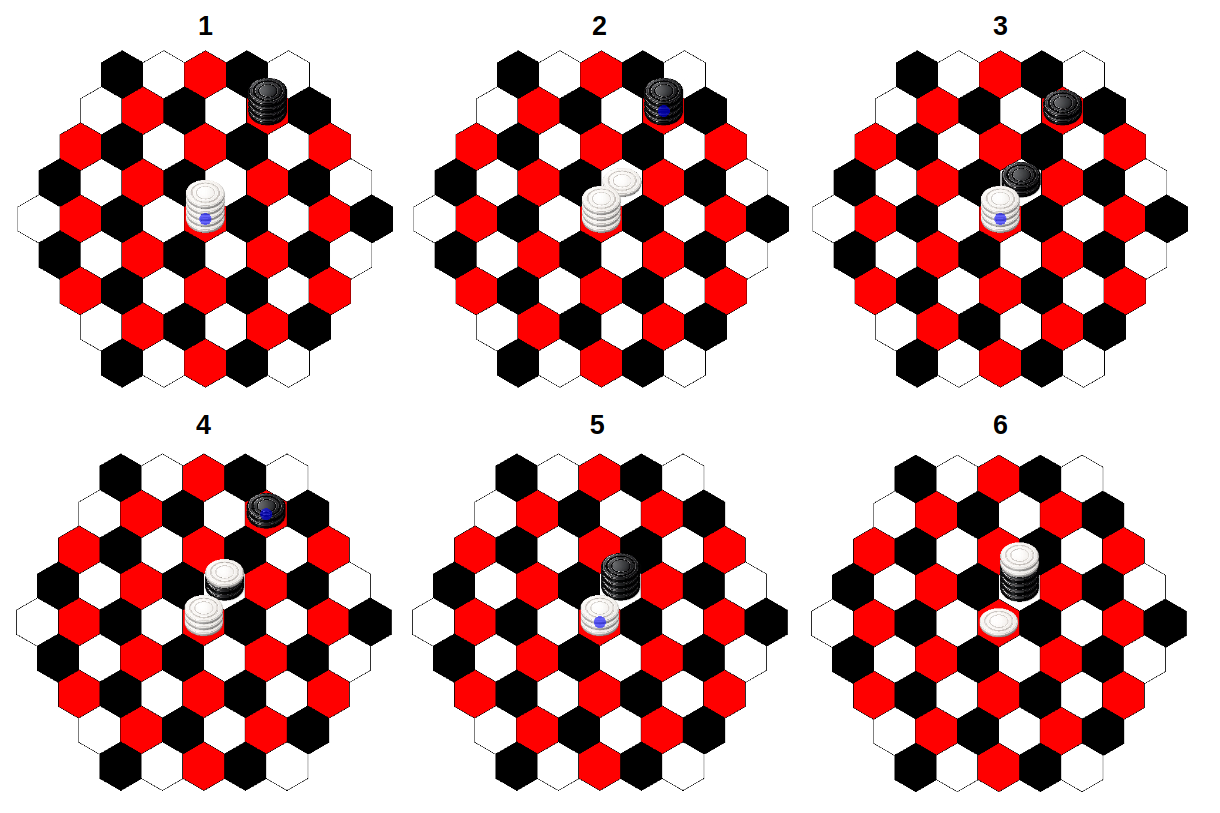
\includegraphics[scale=0.3]{advanced_ai_agents/images/diverse_figures/single_pawn_baiting.png}
    \caption{Figure displaying how the "single piece baiting" strategy used by the white player defeats the powerful stack of the black player.}
    \label{fig:single_pawn_baiting}
\end{figure}

In the scenario presented in Figure \ref{fig:single_pawn_baiting}, the white player (which we will refer to as "White") has a stack of 5 pieces on the red central tile and the black player (which we will refer to as "Black") has a stack of 4 pieces on a red tile close to White. In the second image, White moves a white piece on a white tile, which forces the Black to capture it with at least 2 pieces (because the tile is at distance 2 of their stack). White then repeats the "single piece baiting" strategy until Black runs out of pieces. Finally, in the sixth image, White manages to imprison all of Black's pieces and wins the game \footnote{Notice that White still has one piece left on the initial central tile, which means this strategy also works when both players have stacks of the same size.}. The reason why this strategy works is because the "victim" player (in this case Black) is further away from the contested tile the attacker (in this case White) initially moved its piece to. Now, the question is, can a stack with less pieces win against a stack with more pieces using a "single piece baiting" attack ? The answer is \textbf{no}.\\

\textbf{Proof}:\\
First, we are only interested in positions where both stacks are on red tiles. This is because during a game, good players will try to move their pieces on the red tiles as fast as possible. Also, we are only interested in positions where the tile used as bait has the color white. This is because using a black or red tile as bait will give the defender the advantage of having a better defended stack, which will force the attacker to use even more pieces to continue the attack. By the geometry of the board, which has a hexagonal tiling, we can observe that for any tile, all the tiles at distance 3 have the same color (see Figure \ref{fig:all_tiles_are_red_at_dist_3} as an example). This means a stack on a red tile can't be attacked with a "single piece baiting" attack using a bait tile at distance 3 of the defender. In the best case, such an attack will happen when using a white bait tile at distance two (e.g. in Figure \ref{fig:single_pawn_baiting} where the white bait tile is at distance two of the black stack).

\begin{figure}[h]
    \centering
    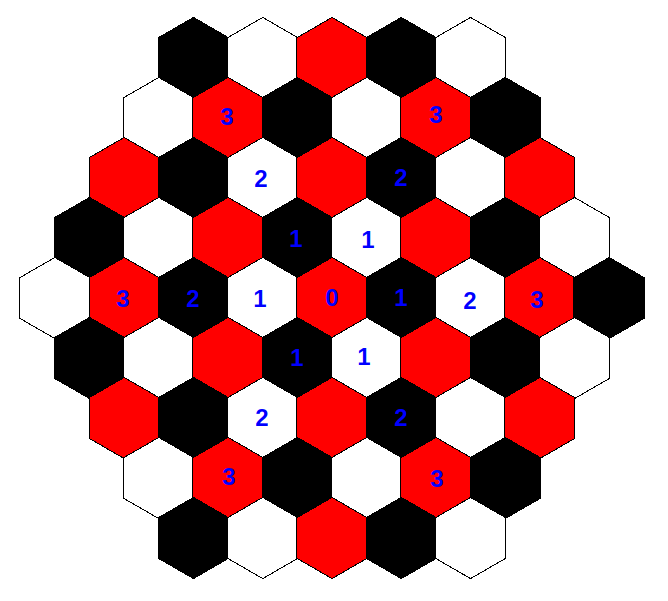
\includegraphics[scale=0.3]{advanced_ai_agents/images/diverse_figures/all_tiles_are_red_at_dist_3.png}
    \caption{Figure showing that all the tiles at distance 3 of the central red tile are also red.}
    \label{fig:all_tiles_are_red_at_dist_3}
\end{figure}

Now that we established the scenarios we are interested in for the "single piece bait" attack, let's show that if the attacker has less pieces than the defender, the attack will never succeed. The following flowchart \ref{fig:schema_single_pawn_bait} proves it by enumerating all the possible moves the attacker has.

\begin{figure}[h]
    \centering
    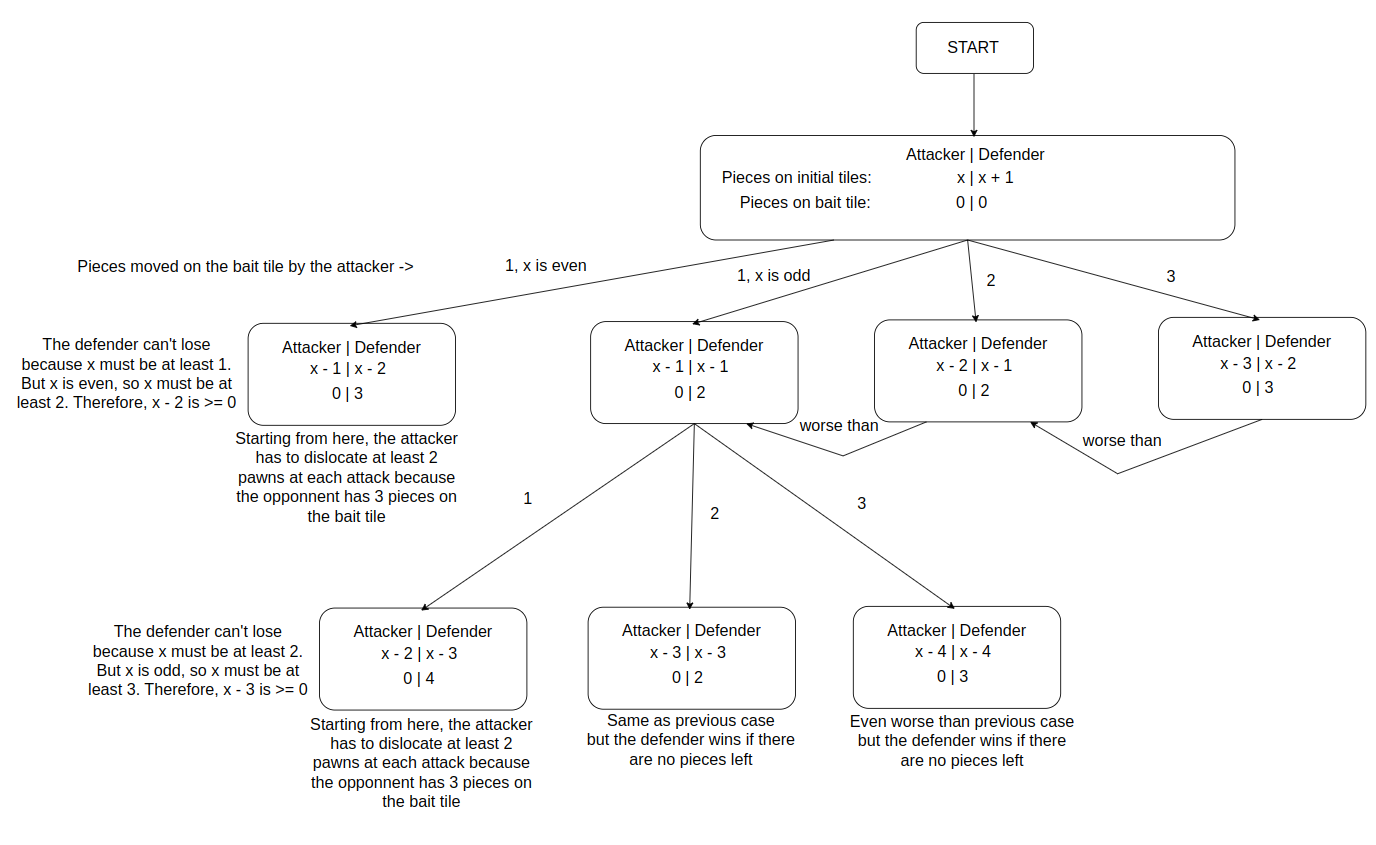
\includegraphics[scale=0.2]{advanced_ai_agents/images/diverse_figures/schema_single_pawn_bait.png}
    \caption{Flowchart of all possible move sequences during a "single pawn bait" attack.}
    \label{fig:schema_single_pawn_bait}
\end{figure}

Finally, a third heuristic is to prioritize stacking pieces on a minimal number of tiles. This is because having a smaller number of big stacks is better than having a bigger number of small stacks. As we just proved earlier, a big stack on a red tile won't be the victim of "single piece bait" attack of a smaller stack, but the opposite is true.

\section{Combined Heuristic and Limitations}

The heuristic evaluation used in this thesis combines the previous observations in a prioritized way. The first priority is the comparison of controlled material, since control of pieces directly affects mobility and the possibility of winning. The second priority is positional power, which rewards control of stronger tiles and more powerful stacks. Finally, the evaluation favors positions where pieces are grouped into stronger stacks rather than being spread across many weak stacks.

This prioritization is important. If positional power were weighted too strongly, an agent might sacrifice too many pieces only to occupy stronger tiles. Such behavior may improve the position locally, but it can be strategically poor if it reduces long-term control and mobility. Giving priority to material control helps avoid this problem.

The proposed heuristic remains handcrafted and therefore limited. It does not capture all tactical motifs of Tricolor, and its weights are not learned automatically from data. Moreover, some strategic features may only become visible through stronger self-play or deeper search. Nevertheless, the heuristic provides a useful first evaluation function for the Alpha-Beta agent introduced in the next chapter.

Future work could investigate automatic heuristic tuning or learning-based evaluation functions. This would be consistent with previous work on heuristic prediction in general game playing, where game descriptions are used to estimate which heuristic features are likely to perform well~\cite{stephenson2021heuristic}. In the case of Tricolor, such approaches could eventually help refine or replace the manually designed evaluation function.